\documentclass[11pt,letterpaper]{article}
\usepackage[margin=1in]{geometry}
\usepackage{amsmath,amssymb,amsthm,graphicx}
\usepackage[hidelinks]{hyperref}
\setlength{\emergencystretch}{2em}
\newtheorem{theorem}{Theorem}
\newtheorem{lemma}[theorem]{Lemma}
\newcommand{\E}{\mathbb E}
\newcommand{\Prb}{\mathbb P}
\DeclareMathOperator{\Bin}{Bin}
\title{A binomial mean of the sum of divisors}
\author{Pioneer project}
\date{28 November 2026}
\begin{document}
\maketitle
\begin{abstract}
For the divisor sum $\sigma$ we prove
$\sum_{k=0}^{n}\binom{n}{k}\sigma(n+k)
=2^n\{\pi^2 n/4+O(\sqrt n\log(2n))\}$.
This proves the asymptotic conjectured by V. Kot\v e\v sovec in OEIS A181411.
The same argument gives an explicit error for shifted, biased binomial means.
It uses only the elementary summatory estimate for $\sigma$ and the variation
of a unimodal probability mass function.
\end{abstract}

\section{The question}
P. D. Hanna's sequence A181411 begins $4,18,55,150,379$ \cite{entry}.
Its $n$th term, for $n\ge1$, is
\[
 A_n=\sum_{k=0}^n\binom{n}{k}\sigma(n+k),\qquad
 \sigma(m)=\sum_{d\mid m}d.
\]
Kot\v e\v sovec conjectured in 2020 that $A_n/(n2^n)$ tends to $\pi^2/4$.
Averaging over a binomial window of width on the order of $\sqrt n$ suffices
even though individual values of $\sigma(m)/m$ fluctuate with the prime factors of $m$.

\begin{theorem}\label{th:main}
Put $c=\sum_{j\ge1}j^{-2}=\pi^2/6$ \cite{basel}. Suppose $h,n$ are positive integers,
$0<p<1$, and $K\sim\Bin(n,p)$. For $M=h+n$ one has
\[
 \left|\E\,\sigma(h+K)-c(h+np)\right|
 \le \frac{\sqrt{\pi}\,M\,[\log M+2+c]}
                {2\sqrt{2np(1-p)}}.
\]
In particular $A_n/(n2^n)=\pi^2/4+O(\log(2n)/\sqrt n)$.
\end{theorem}

\section{An explicit discrepancy bound}
Let $R(0)=0$ and $R(m)=\sum_{j=1}^m (\sigma(j)-cj)$.
\begin{lemma}\label{lem:sigma}
For every integer $m\ge1$,
$|R(m)|\le \tfrac12m(\log m+2+c)$.
\end{lemma}
\begin{proof}
Write $T(v)=v(v+1)/2$. Reversing the order of summation gives
$\sum_{j\le m}\sigma(j)=\sum_{d=1}^m T(\lfloor m/d\rfloor)$.
Indeed each positive pair $(d,e)$ with $de\le m$ contributes the divisor $e$.
For $z\ge1$ put $v=\lfloor z\rfloor$. Monotonicity gives
$z(z-1)\le v(v+1)\le z(z+1)$. Thus
\[
 \left|\sum_{j\le m}\sigma(j)-\frac{m^2}{2}\sum_{d=1}^m d^{-2}\right|
  \le \frac m2\sum_{d=1}^m d^{-1}.
\]
Integral comparison bounds the last harmonic sum by $1+\log m$ and
$\sum_{d>m}d^{-2}$ by $1/m$. Subtracting $cm(m+1)/2$ now gives the claim.
\end{proof}

\section{Smoothing by a binomial law}
Write $w_k=\Prb(K=k)$ for $0\le k\le n$, and extend $w_k=0$ to the other
integers. The neighboring ratio
$w_{k+1}/w_k=(n-k)p/((k+1)(1-p))$ decreases in $k$. Hence
\begin{equation}\label{eq:variation}
 \sum_{k=-1}^n|w_k-w_{k+1}|=2\max_k w_k.
\end{equation}
The sum telescopes separately on the two sides of a maximum, including when
there are two adjacent maxima. Fourier coefficient extraction from
$(1-p+pe^{it})^n$ gives, uniformly in $k$,
\[
 w_k\le\frac1{2\pi}\int_{-\pi}^\pi
 (1-4p(1-p)\sin^2(t/2))^{n/2}\,dt
 \le \frac{\sqrt\pi}{2\sqrt{2np(1-p)}}.
\]
For the last inequality use $1-v\le e^{-v}$,
$\sin(|t|/2)\ge |t|/\pi$ on this interval, and integrate the Gaussian
on the real line.

\begin{proof}[Proof of Theorem~\ref{th:main}]
The discrepancy in the theorem is a weighted first difference of $R$.
Summation by parts with the zero extension of $w$ writes it exactly as
\[
 \sum_{k=0}^nw_k\{R(h+k)-R(h+k-1)\}
  =\sum_{k=-1}^n R(h+k)(w_k-w_{k+1}).
\]
Here $h\ge1$, so $R(h-1)$ is defined. Apply Lemma~\ref{lem:sigma} up to
$M$ and use \eqref{eq:variation}. For $h=n$, $p=1/2$, the expectation
is $2^{-n}A_n$ and $c(h+np)=\tfrac32 cn=\pi^2 n/4$.
\end{proof}

\begin{figure}[h]
\centering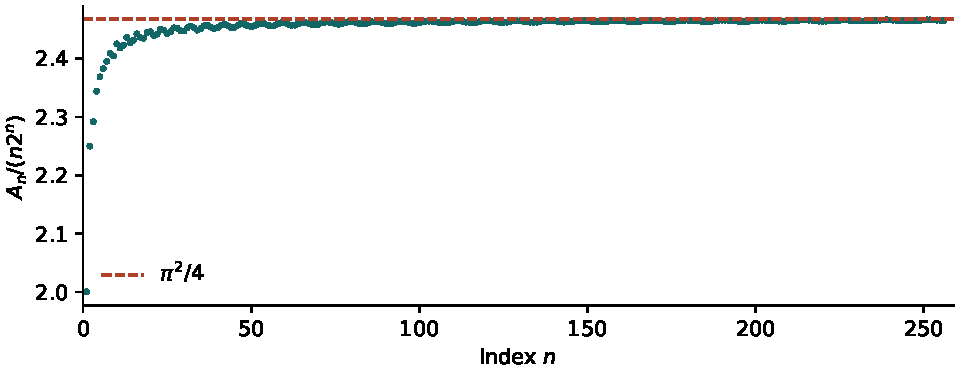
\includegraphics[width=.80\linewidth]{mean.pdf}
\caption{The normalized exact divisor sums for $1\le n\le256$. The dashed line
is $\pi^2/4$. The integer numerator and denominator are evaluated before
conversion for plotting.}\label{fig:data}
\end{figure}
\begin{thebibliography}{9}
\bibitem{entry} P. D. Hanna, \emph{A binomial sum of the divisor function},
OEIS A181411 (2010), with V. Kot\v e\v sovec's conjecture (2020).
\url{https://oeis.org/A181411}.
\bibitem{basel} L. Euler, \emph{De summis serierum reciprocarum},
Commentarii Academiae Scientiarum Petropolitanae 7 (1740), 123--134.
\url{https://scholarlycommons.pacific.edu/euler-works/41/}.
\end{thebibliography}
\end{document}
